\begin{event}
  {GAP--Singular School and Meeting}
  {TODO}  % {eventId}
  {PfalzAkademie, Lambrecht, Germany, 15--23 August, 2019}
  {TODO}  % {Partners (use Partners id, separated with coma)}
  {33}
  {TODO}  % {nb of ODK participants}
  {https://opendreamkit.org/meetings/2019-04-02-GAPSingularMeeting/}

\textbf{Main goals.}
The main goals were to introduce beginners to \GAP and \Singular, present
computer algebra--related work, and share ideas through workshops.

\textbf{ODK implication.}
\TODO{Describe how ODK was involved and give a rough estimation of cost for ODK}

\textbf{Event summary.}
The event consisted of three parts:
\begin{itemize}
\item School: a sequence of workshops to introduce beginners to \GAP, \Singular,
  and open-source development principles.
\item Mini-conference: talks to allow participants to present computer
  algebra--related work to each other.
\item Workshops: a set of workshops dedicated to specific computer algebra
  problems.
\end{itemize}

\textbf{Demographics.}
\TODO{Do you have demographic information? If so, please share!}

\textbf{Results and impact.}
In the School, tutorials were given that introduced participants to:
\begin{itemize}
\item Best practices in software development (Max Horn);
\item Basic use of \GAP (Michael Torpey);
\item Advanced Topics in \GAP (Thomas Breuer);
\item Basic use of \Singular (Christian Eder, Andreas Steenpaß, Isabel Stenger);
\item Parallel modular algorithms in Singular (Christian Eder, Andreas Steenpaß, Isabel Stenger);
\item CAP: Categories, algorithms, programming (Sebastian Posur).
\end{itemize}
These tutorials were complemented by informal discussions, and chances for
learners to answer questions.  The ``Best practices'' and ``Basic use of \GAP''
sessions followed material from appropriate Software Carpentry courses
(\url{https://software-carpentry.org/lessons/}): ``Version Control with Git''
and ``Programming with GAP'' respectively.

\TODO{What did you achieve with this event? (If ever it impacted 
other ODK tasks and deliv, mention it here) \qquad MT: I wrote about the School,
which is the bit I was there for.  More description should probably be included
about the bits that came later on.}

\begin{figure}[ht]
  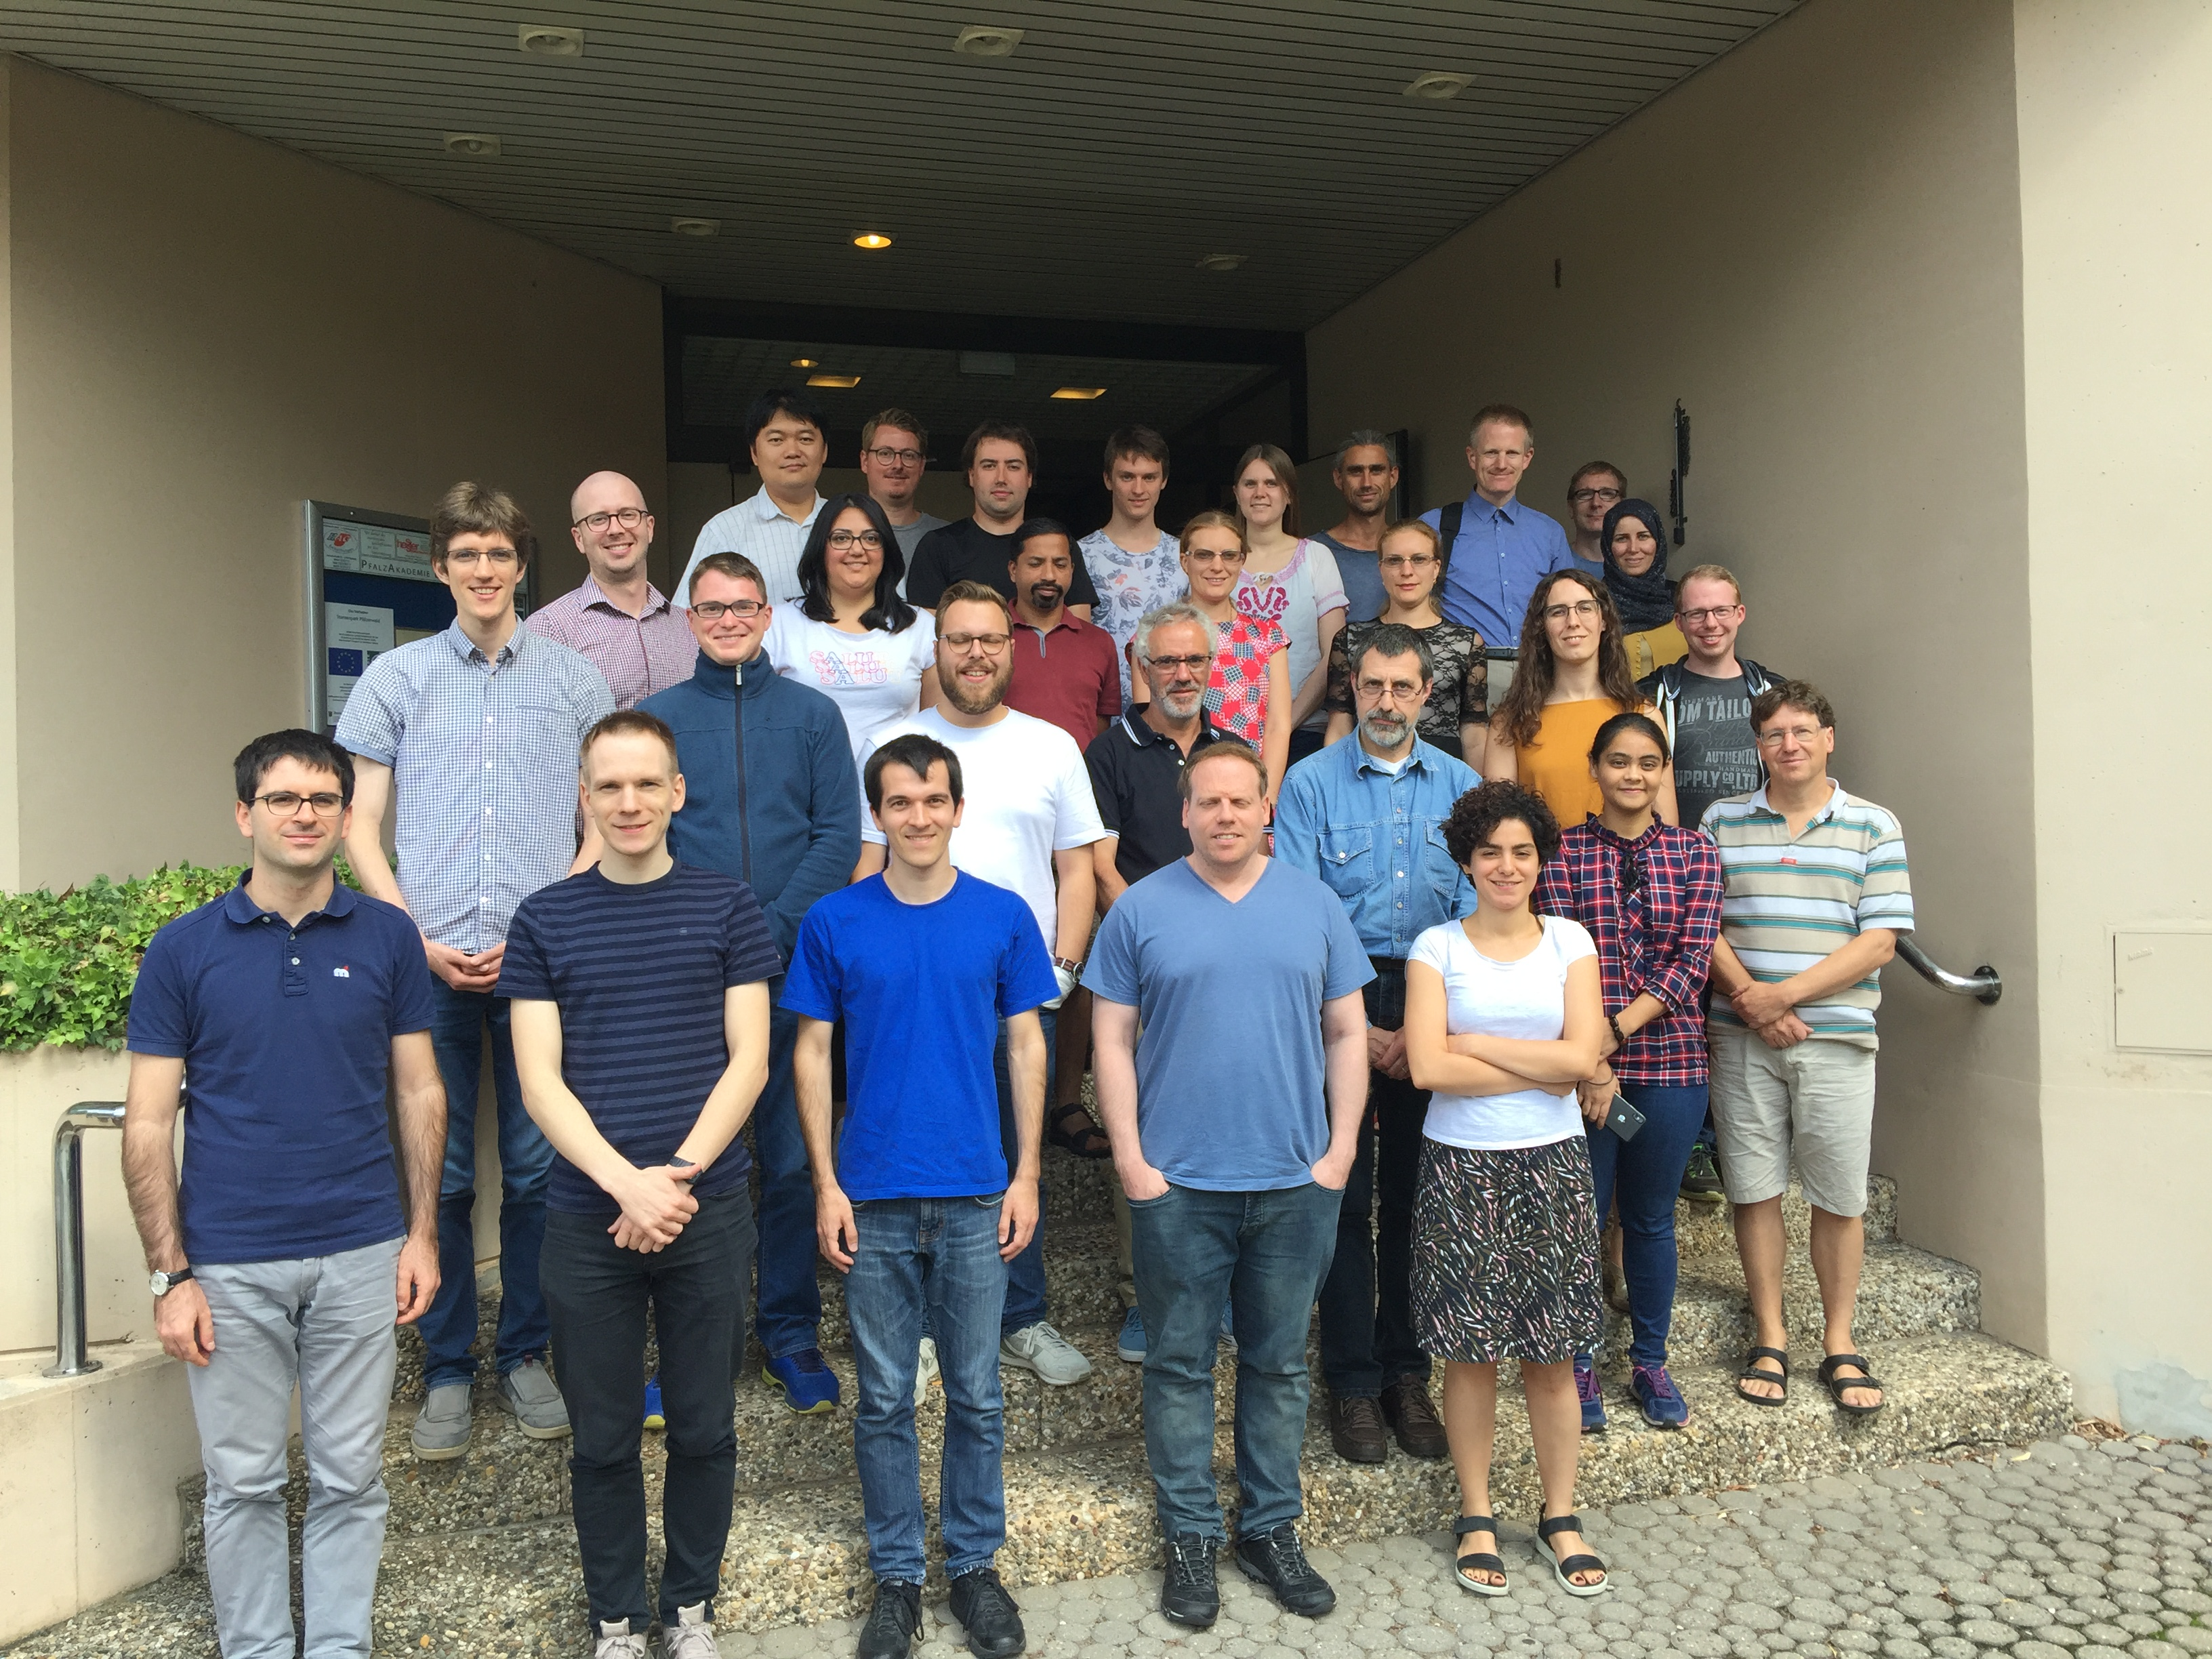
\includegraphics[width=\textwidth]{gap-singular-participants}
  \caption*{Conference photo of GAP--Singular meeting}
\end{figure}

\end{event}
